% !TEX root = ../main.tex
\subsubsection{Electron Variables}
\label{14.21::electron_variables}
    % Electron variables.
    The acceptance of the scattered electron variables $Q^2$ and $\nu$ are presented in Figure \ref{fig::14.12::electron_acc}.
    Each one is presented in integrated kinematical region for the other variable.

    \begin{figure}[t!]
        \centering
        % Q2.
        \begin{subfigure}[b]{\textwidth}
            \centering
            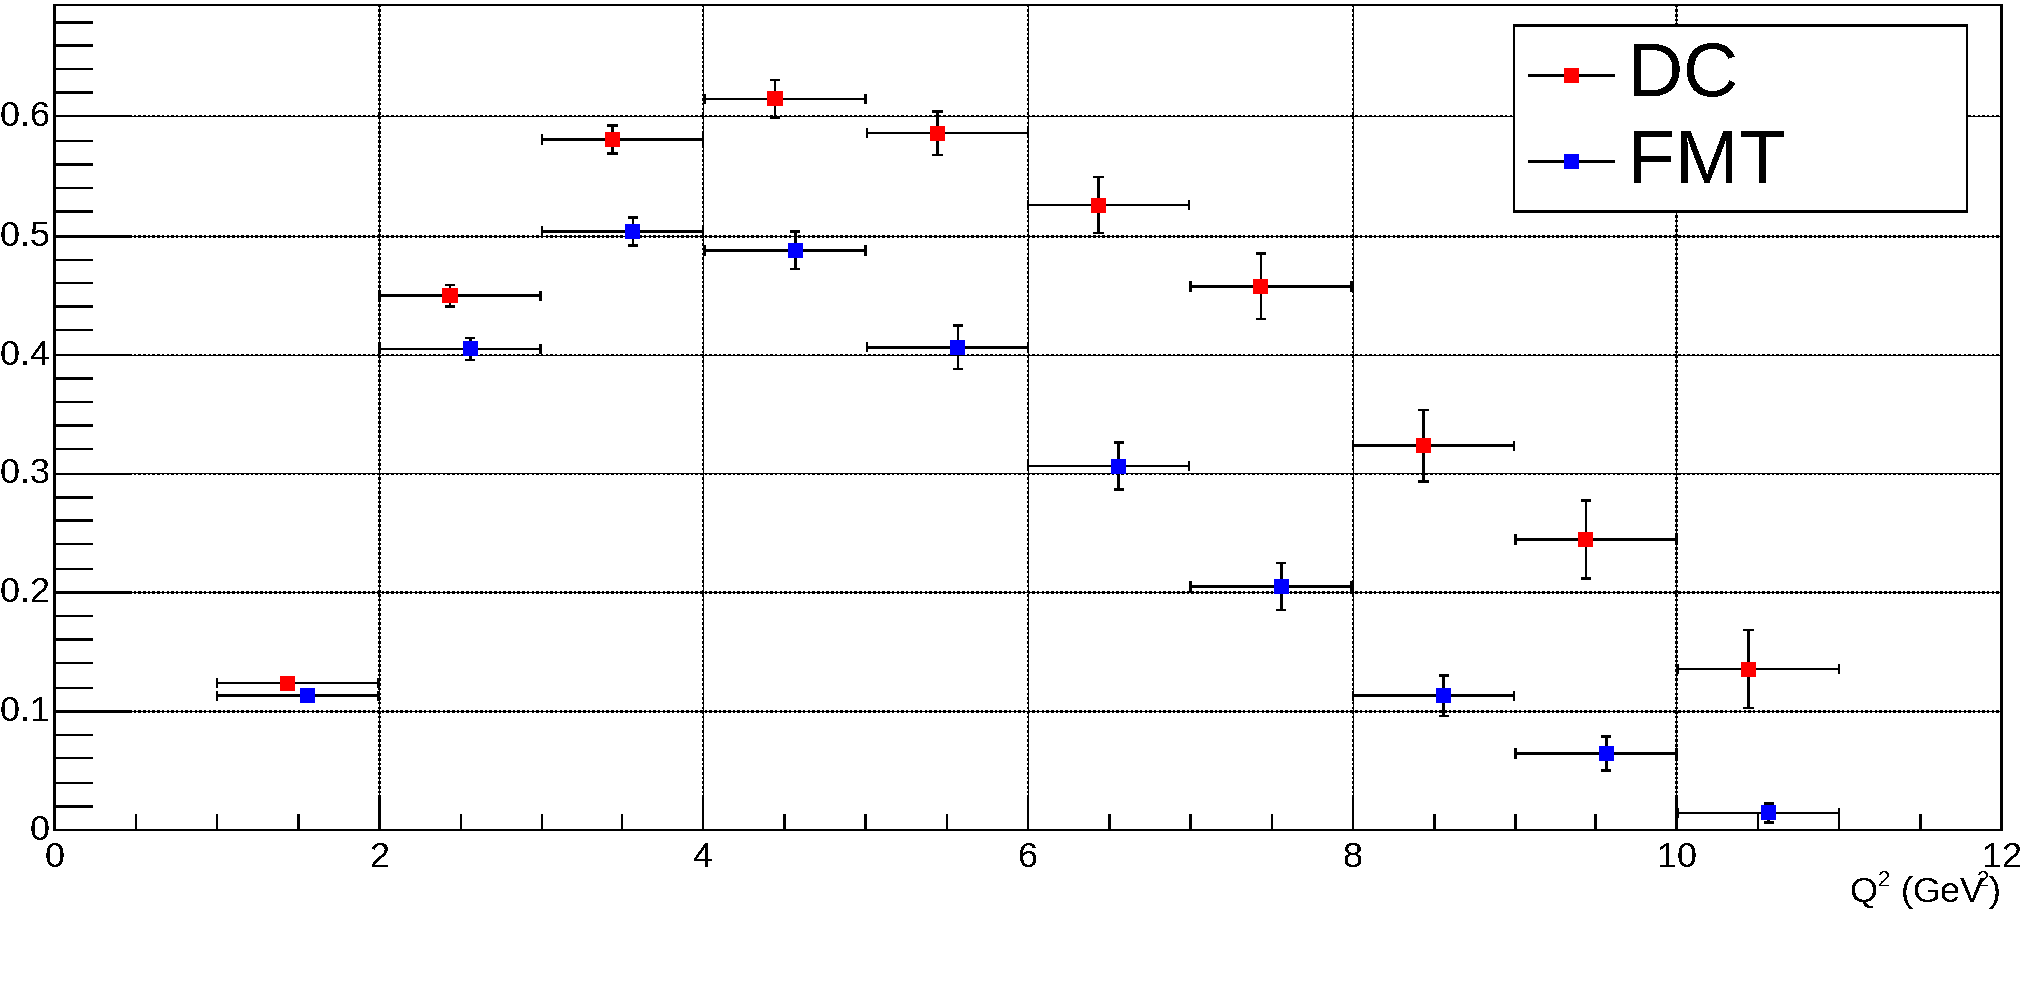
\includegraphics[width=\textwidth]{21q2_acc.pdf}
            \caption{$Q^2$ acceptance.}
            \label{fig::14.21::q2_acc}
        \end{subfigure}
        \hfill
        % nu.
        \begin{subfigure}[b]{\textwidth}
            \centering
            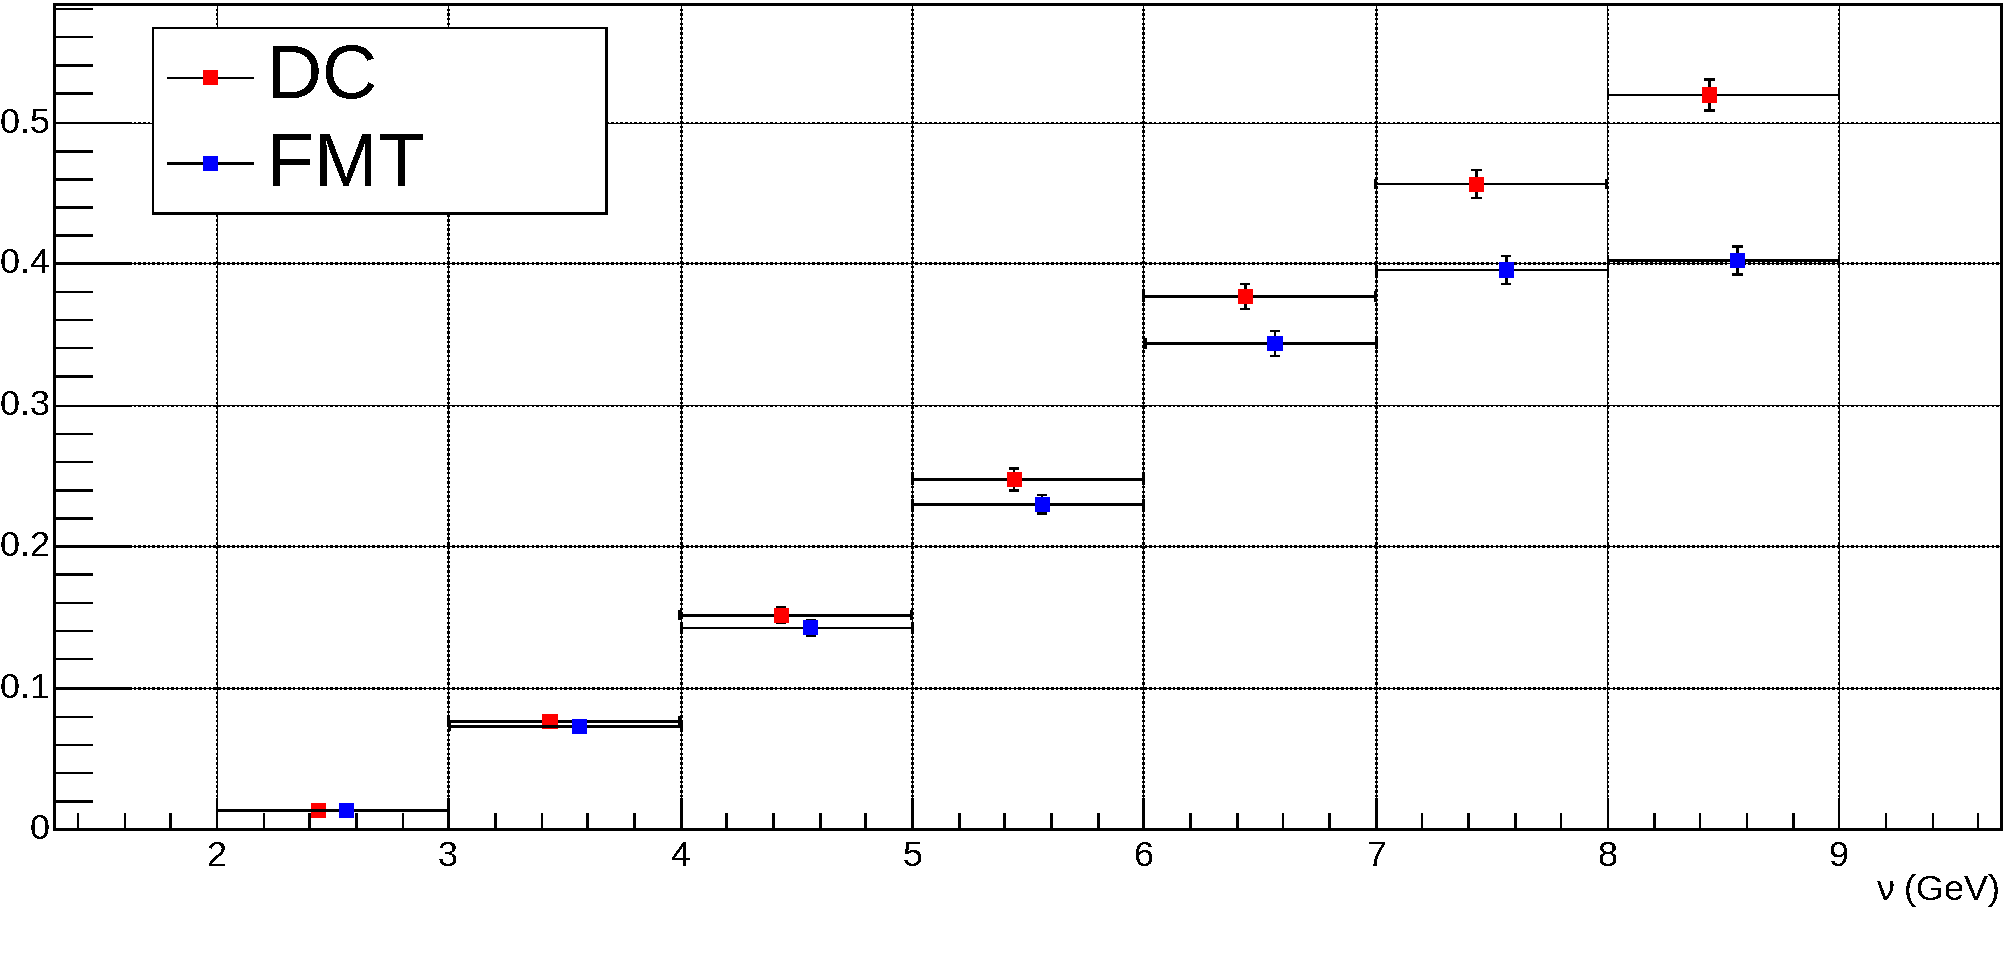
\includegraphics[width=\textwidth]{21nu_acc.pdf}
            \caption{$\nu$ acceptance.}
            \label{fig::14.21::nu_acc}
        \end{subfigure}
        \caption[$e^-$ variables acceptance]
        {$e^-$ variables acceptance.
        $\nu$ is integrated in \ref{fig::14.21::q2_acc}, and $Q^2$ is integrated in \ref{fig::14.21::nu_acc}.
        The bin markers are slightly shifted in $x$ to improve legibility.}
        \floatfoot{Source: Own elaboration, using the \href{https://github.com/bleaktwig/clas12-rge-analysis}{clas12-rge-analysis} software.}
        \label{fig::14.21::electron_acc}
    \end{figure}

    \begin{figure}
        \centering
        % phi vs theta.
        \begin{subfigure}[b]{\textwidth}
            \centering
            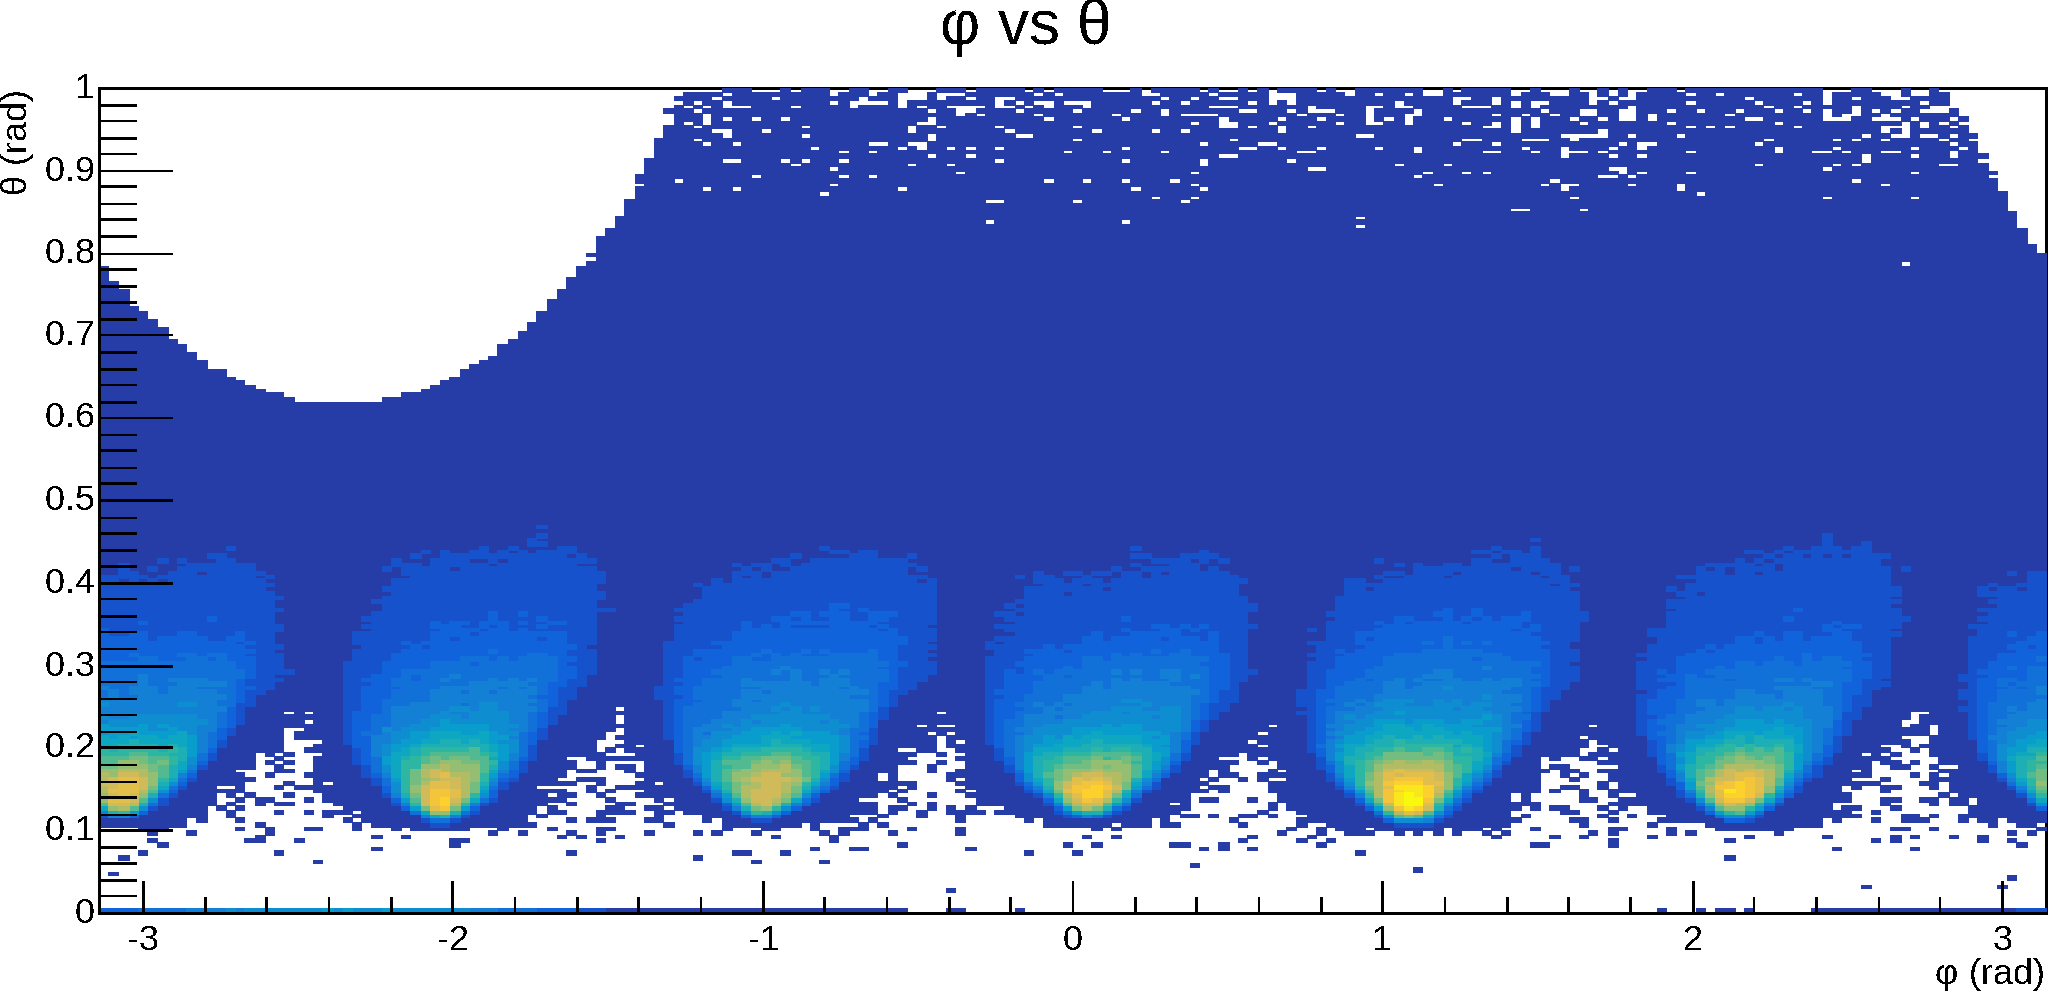
\includegraphics[width=\textwidth]{21phi_theta_neg.pdf}
            \caption[$\phi$ vs $\theta$ for negative particles]
            {$\phi$ vs $\theta$ for negative particles detected by DC.
            The sector with less acceptance than the rest is caused by \textbf{TODO}.}
            \label{fig::14.21::phi_theta_neg}
        \end{subfigure}
        % theta.
        \begin{subfigure}[b]{\textwidth}
            \centering
            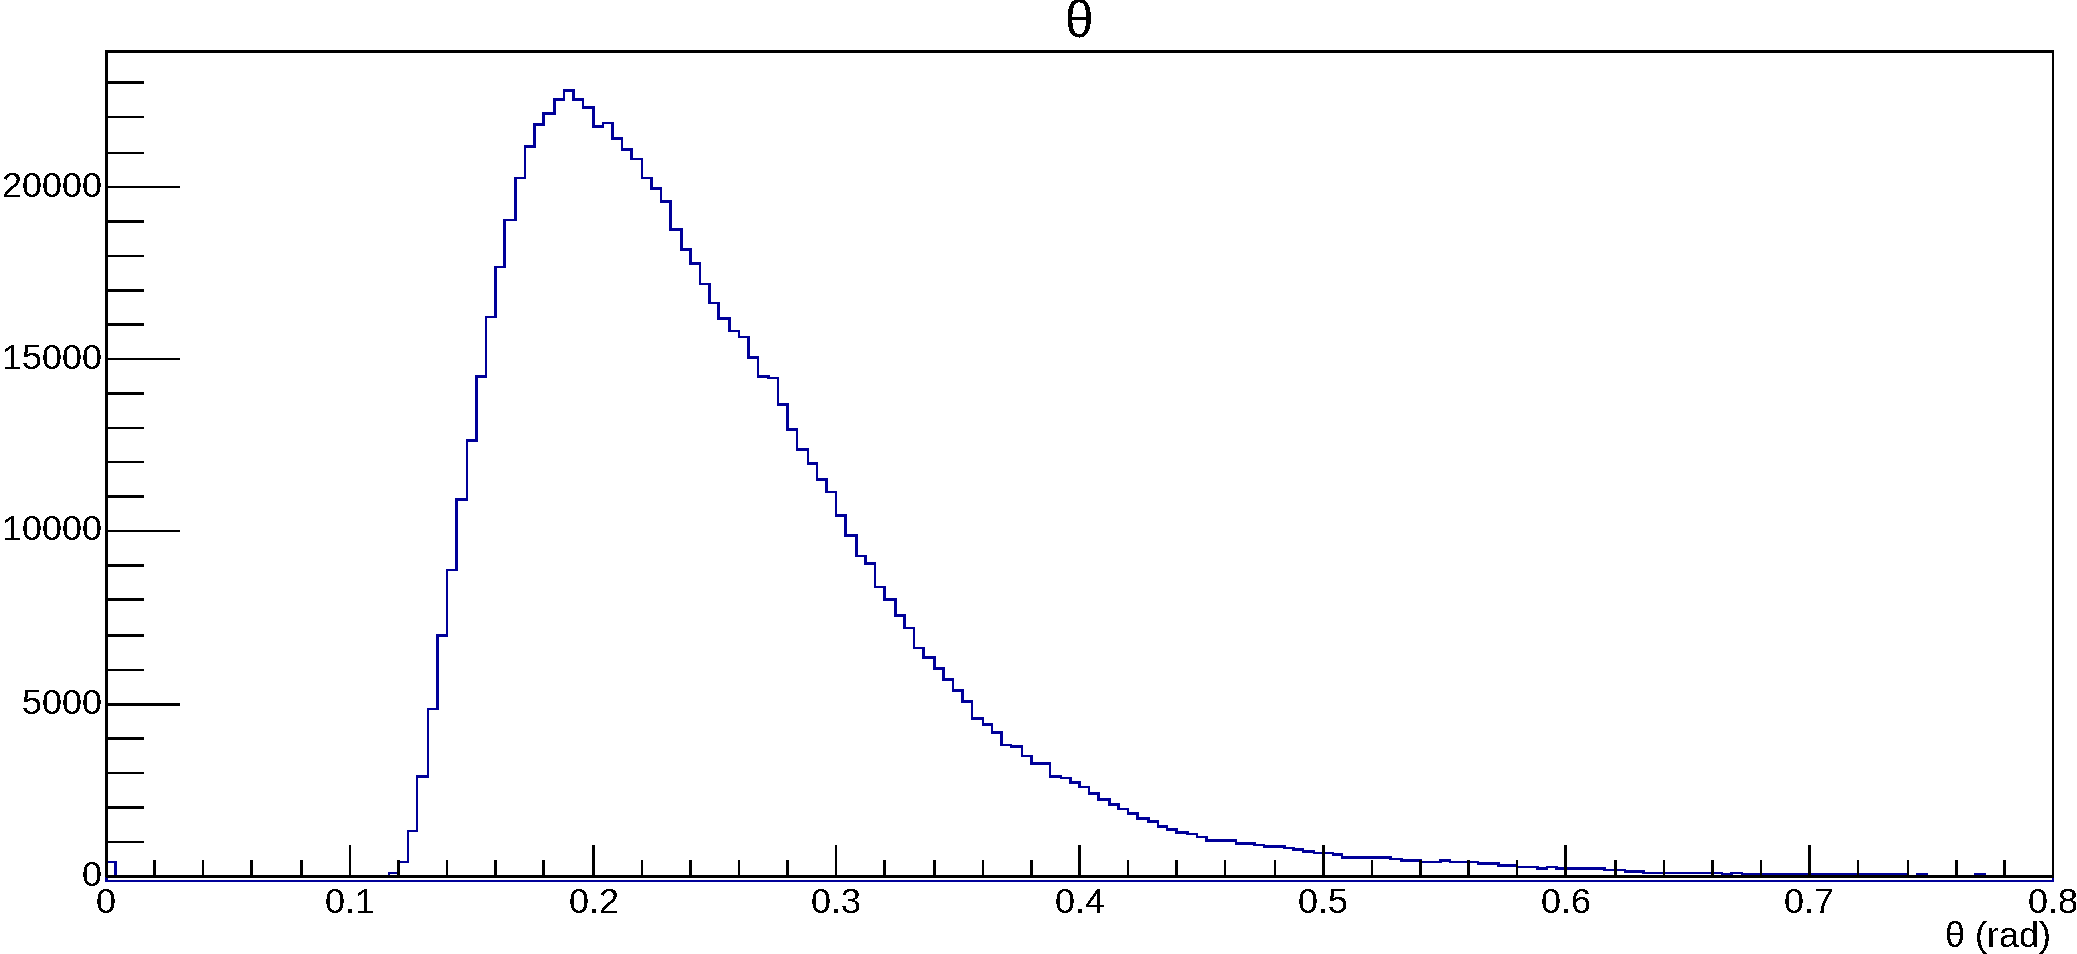
\includegraphics[width=\textwidth]{21theta_neg.pdf}
            \caption[$\theta$ for negative particles]
            {$\theta$ for negative particles detected by DC.}
            \label{fig::14.21::theta_neg}
        \end{subfigure}
        \caption[$\theta$ study for negative particles]
        {$\theta$ study for negative particles.
        Simulated data.}
        \floatfoot{Source: Own elaboration, using the \href{https://github.com/bleaktwig/clas12-rge-analysis}{clas12-rge-analysis} software.}
        \label{fig::14.21::theta_study_neg}
    \end{figure}

    % Q2.
    As can be seen in Equation \eqref{eq::13.23::q2}, $Q^2$ depends quadratically on the $\theta_C$ of the scattered electrons (for small angles).
    Therefore, it's useful to understand the $\theta$ acceptance of CLAS12, such that we can disentangle this geometric effect from the inherent $Q^2$ acceptance of the FD.
    We can see this dependance for negative particles in Figures \ref{fig::14.21::phi_theta_neg} and \ref{fig::14.21::theta_neg}.

    The triangular shape of each DC sector in conjunction with the inbending tracks from the negative solenoid field leads to a very low acceptance at low $\theta$ angles.
    Integrating across $\phi$, this causes a low $\theta$ efficiency for $\theta \lsim 0.15$ radians.
    Looking back at $Q^2$ in Figure \ref{fig::14.21::q2_acc}, the drop in $Q^2$ acceptance between 1 and 4 $GeV^2$ can be clearly correlated with this effect -- it is purely geometric in nature.

    % nu.
    Since $\nu$ presents no direct correlation with $\theta_C$ (See Equation \eqref{eq::13.23::nu}), we can assume that the acceptance we see in Figure \ref{fig::14.21::nu_acc} is intrinsic to the detector.
